\documentclass{sbrt2018port}

\usepackage{flushend}

\begin{document}

\title{Título do Trabalho}

\author{ Matheus Bazzo \\
Prof.ª: Juliana Camilo Inácio}

\maketitle

\markboth{UNIVERSIDADE DO OESTE DE SANTA CATARINA - CURSO DE ENGENHARIA DE COMPUTAÇÃO, SISTEMAS E REDES DE TELECOMUNICAÇÕES, 2018/2} {UNIVERSIDADE DO OESTE DE SANTA CATARINA - CURSO DE ENGENHARIA DE COMPUTAÇÃO, SISTEMAS E REDES DE TELECOMUNICAÇÕES, 2018/2}

\begin{resumo}
O resumo sobre o tema do trabalho vai aqui. O resumo deve incluir, mais ou menos 200 palavras.
\end{resumo}

\begin{chave}
Celulares, Histórico, Mercado, Telefonia móvel, Telecomunicações.
\end{chave}

\section{Introdução}

O primeiro telefone foi criado por alexander graham bell em 1875, dando início a tudo o que conhecemos hoje em termos de comunicação a distancia, no brasil não demorou muito para chegar, apenas dois anos após a criação, dom pedro II trouxe para sua casa o telefone.
Em 1879 é feita a primeira conexão nacional, e por consequencia nasceu a primeira empresa de telefonia brasileira a "Telephone Company of Brazil", nessa época as ligações não eram diretas, ficando a cargo das "telefonistas" fazerem a interligação manualmente por cabos.
Em 1997 a telebrás, empresa brasileira de telecomunicação é dividida, dando origem a mais doze empresas, é iniciado o processo de privatização das telecomunicações no brasil, com a lei LGT, posteriormente a isso nasce a ANATEL, empresa reguladora de telecomunicações no brasil.
Enquanto isso no mundo, em 1994 é criado pela IBM o primeiro celular com algumas funções alem da conversação, como, email e agenda, nasce o que conhecemos hoje por Smartphone.

\section{Mercado das Telecomunicações no Brasil}
\label{s_mercadoBrasil}
Logo após a criação da LGT, em 1997, se começou a criar um monopólio por volta de 2006, onde existiam apenas três grandes empresas de telecomunicações, CLARO, TIM e VIVO, e até hoje esse cenário não mudou muito, tendo apenas algumas mais regionais, não é atoa que o brasil tem os serviços de telefonia mais caros do mundo, segundo a UIT, União Internacional das Telecomunicações, o brasil é o 4º mais rentável do mundo em telecomunicações, mas muitas vezes não é pelo consumo e sim pelo custo.
Já o cenário de provedores de internet é mais abrangente, principalmente em questão regional, onde é mais barato e facil vender internet fixa à população, hoje o brasil conta com 5.7 mil provedores de internet espalhados pelo país.
Mas o setor de telecomunicações não tem apenas esses dois setores, o mesmo é divido em 6 segmentos entre eles: Telefonia Fixa, Comunicação Móvel, Comunicação Multimídia, TV por Assinatura, Radiodifusão entre outros serviços

\subsection{Seguimento escolhido}
\label{s_segmento}

Nessa seção você deve:
\begin{enumerate}
    \item Se aprofundar nas informações desse segmento;
    \item Colocar informações interessantes e que ache necessária;
    \item Imagens, gráficos e tabelas enriquecem o trabalho (e não são restritos a essa seção apenas), mas apenas utilize esses recursos se você tiver algo para comentar sobre eles.
\end{enumerate}


\begin{figure}[!ht]%[!htpb]
    \centering
    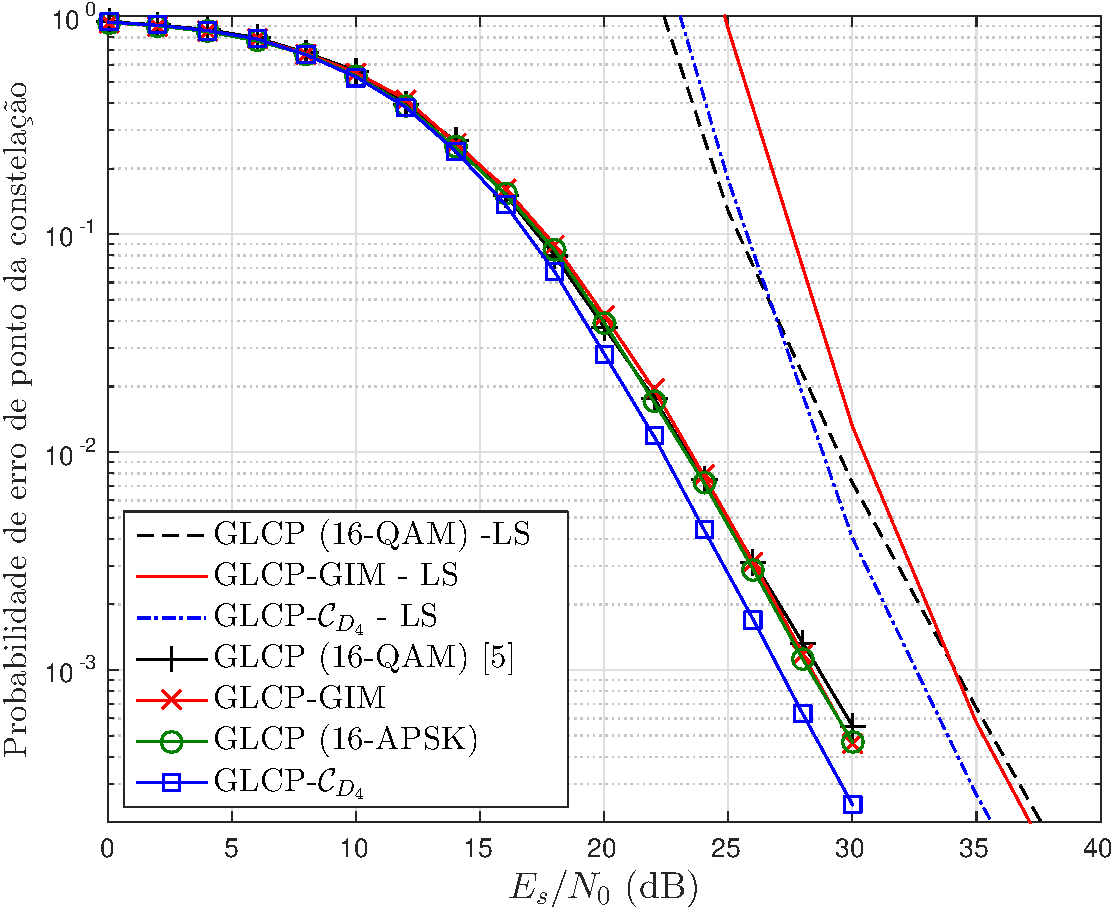
\includegraphics[width=\linewidth]{CER_schemesD2.pdf}
    \caption{Exemplo de inserção de figura.}
    \label{f_cerd2}
\end{figure}

\section{Conclusões}
\label{s_concl}

Aqui você vai concluir o trabalho. Tente não copiar as informações colocadas aqui. O ideal é que você leia e escreva com as suas palavras o que entendeu sobre o assunto. O texto como um todo deve estar coerente. O trabalho deve ter no máximo 2 páginas, ou seja, uma folha frente e verso. Um material de apoio será disponibilizado com informações sobre como escrever um artigo científico segundo as normas da IEEE entre outras coisas.


\begin{thebibliography}{99}
\bibitem{sim2013}
E.~Basar, U.~Aygolu, E.~Panayirci and H.~V.~Poor, ``Orthogonal Frequency Division Multiplexing With Index Modulation,'' \emph{IEEE Trans. Signal Process.}, vol. 61, no. 22, pp. 5536--5549, Nov. 2013.

\bibitem{isim2014}
Y.~Xiao \emph{et al.}, ``OFDM with Interleaved Subcarrier-Index Modulation,'' \emph{IEEE Commun. Lett.}, vol. 18, no. 8, pp. 1447--1450, Aug. 2014.


\bibitem{tsebook}
D.~Tse and P.~Viswanath, \emph{Fundamentals of Wireless Communications}, Cambridge, U.K.: Cambridge, Univ. Press, 2005.

\bibitem{lattice}
J.~H.~Conway and N.~J.~A.~Sloane. \emph{Sphere Packings, Lattices and Groups}, 3rd Edition, Springer-Verlag, 1999.

\bibitem{3gpp_eva}
\emph{User Equipment ({UE}) Radio Transmission and Reception. Technical Specification Group Radio Access Network; Evolved Universal Terrestrial \hspace*{0.55cm} 
Radio Access ({E-UTRA})}, 3GPP TS 36.101, Apr. 2017. 

\end{thebibliography}


\end{document}
